\documentclass[a4paper, openany]{memoir}

\usepackage[utf8]{inputenc}
\usepackage[T1]{fontenc} 
\usepackage[english]{babel}
\usepackage{amsmath}
\usepackage{amssymb}

\usepackage{booktabs}
\usepackage{fancyhdr}
\usepackage{float}
\usepackage{indentfirst}
\usepackage{graphicx}
\usepackage[linewidth=1pt]{mdframed}
\usepackage{multicol}
\usepackage{fancyvrb}

\pagestyle{fancy}
\fancyhf{}
\fancyhead[LE]{\leftmark}
\fancyhead[RO]{\rightmark}
\fancyhead[RE, LO]{PSD}
\fancyfoot[LE, RO]{\thepage}
\fancyfoot[RE, LO]{Pete Gautam}

\renewcommand{\headrulewidth}{1.5pt}

\chapterstyle{thatcher}
\setcounter{chapter}{8}

\begin{document}
\chapter{Continuous Integration}

Integration hell refers to the situation where a software developer spends more time trying to re-integrate altered source code into a software system than creating the feature. This situation can occur as the software evolves, and even when we use source code management systems. This is because other developers have concurrently made changes that may prevent the software system from compiling, or cause some of its tests to fail. Moreover, it can also cause conflicts with the new features that the developer has built.

These problems tend to be exacerbated when a developer tries to integrate a very large change to the source codebase in one go, or when new features are integrated infrequently or late. These factors are linked- very large changes to the software system often involve a considerable greater amount of work, meaning longer periods between reintegration of software into the main source codebase.

\section{Continuous Integration Practices}
Continuous integration is a set of practices as a means of mitigating continuous and concurrent software development efforts within a team. A number of practices for continuous integration exist, such as change management, quality assurance and deployment.

In change management, the follows are the recommended practices:
\begin{itemize}
    \item the team should maintain a single source repository that everybody commits to.
    \item everyone should commit to the mainline (master branch) every day.
    \item every commit should build the mainline on an integration machine. This allows the commit to be tested, which shows that it can be compiled. Moreover, we can run some unit tests and static analysis at the same time.
    \item everyone should be able to see what is happening in the single source code repository to maintain transparency.
\end{itemize}
In terms of quality assurance:
\begin{itemize}
    \item the build process for each commit should be automated.
    \item the build should be self-testing, i.e. it should have a unit test suite that can be executed on every commit.
    \item the test suite should be deployed in a clone of the production environment so that the testing is accurate. The build should be kept fast, typically within 10 minutes.
\end{itemize}
In terms of deployment:
\begin{itemize}
    \item it should be easy for anyone to get access to the latest executable. The build should be compiled automatically and published for access to anyone who wants it.
    \item the deployment of code should be automated into a production environment to make it part of the delivery pipeline.
\end{itemize}

\subsection{Integration Frequency}
Many software projects adopt a late integration strategy when integrating new features. This means that the developers in the project each work on a separate branch (copy of the project source code) to implement new features during the course of the sprint. As each developer completes a new feature towards the end of the sprint, they submit their changes to code.

Unfortunately, because everyone else also wants to reintegrate changes at the same time, there might be a considerable amount of conflict between the new features, and the team might have to spend a lot of time on integration at the end of the sprint.

\begin{figure}[H]
    \centering
    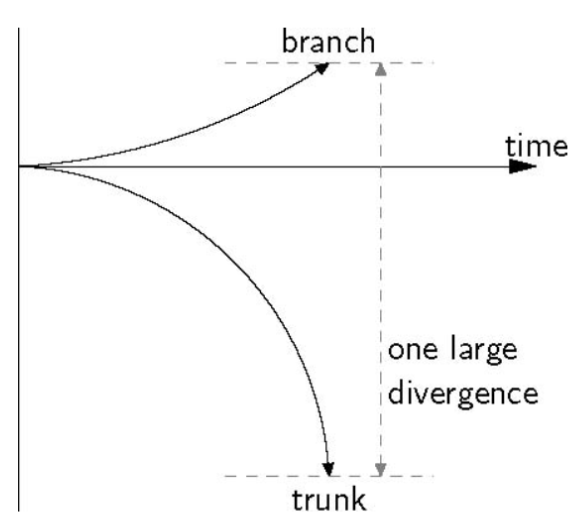
\includegraphics[scale=0.5]{src/9.1 normal integration frequency.PNG}
\end{figure}
\noindent The image above illustrates why late integration creates so much extra work at the end of the sprint. The trunk diverges from the baseline faster than the branch. This is because the trunk represents the effort of every other developer making smaller commits than a whole new feature (such as defect fixes). This means that when a branch is ready to be integrated, there will be a considerable amount of work to do. 

\begin{figure}[H]
    \centering
    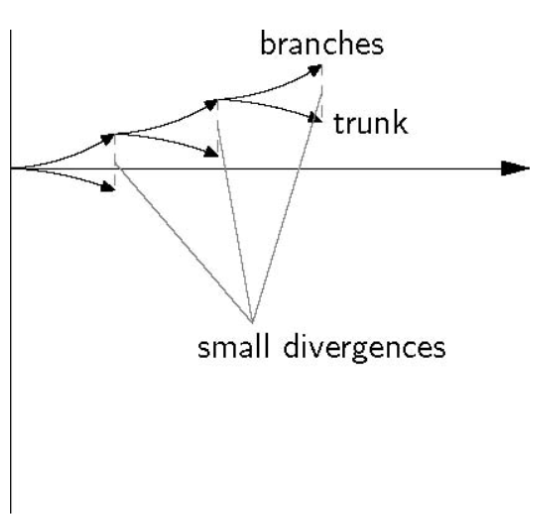
\includegraphics[scale=0.5]{src/9.2 merged integration frequency.PNG}
\end{figure}
\noindent The image above shows the alternative approach for continuous integration. Here, the branch developer devises their work into small chunks so that changes can be integrated much more frequently. As each small new task is completed, it is immediately reintegrated to the trunk. This limits the effect of exponential rate of divergence of the trunk. 

\section{Feature Branching}
In its pure form, CI doesn't permit for branching in a project. All developers should make small, frequent changes to master. Some project teams find this impractical. Feature branches can be a useful way to experiment with longer-term proposals. Permitting the use of branches allows changes to the branch to be maintained within the source repository.

If branches are going to be used in a project managed in CI, there are several compromising strategies in managing the branches and the master branch.
\begin{itemize}
    \item We can implement the new feature on master, with frequent commits of small changes. This is the approach advocated by CI purists.
    
    \item We can implement the new feature in a branch and merge changes from master frequently. This works best for medium-term feature branches that are low on certainty. Merging from master ensures that it never diverges too far from the trunk, while also not affecting the trunk itself.
    
    \item We can implement the feature as a prototype branch and then re-impl-ement the feature on the trunk in small changes rather than merging from the prototype branch into master. This allows the prototype branch to diverge as much as necessary and can be useful in providing sufficient freedom for evaluating high-risk features.
    
    \item We can implement the feature as a permanent branch. This creates a fork of the project within the repository. The branch effectively becomes a separate trunk project for an alternative customer, while still maintaining a substantially similar codebase within the parent project.
\end{itemize}

\subsection{Maintaining multiple CI processes}
We have assumed that each single software project will have a single CI process. However, in a situation where the software project is maintaining a number of different branches, it makes sense to think about maintaining multiple CI processes as well. In fact, the longer the branch lives, the more important it can be to set up a separate CI process for it.

Some larger processes might maintain several different permanent CI pipe-lines for different branches of the project. The master branch is the most important build to monitor and will have new features and defect fixes applied. It might also be useful to set up CI pipelines for forked developments for specific customers or purposes, or the latest stable release that only receives defect fixes. It can also be used in significant feature branches that are long-lived.

In some cases, some software projects apply a CI process to every branch within the project. This is a good way to prevent defects from being introduced to the master branch as we catch them in the development branch.

\section{Detecting broken builds}
Uncontrolled, high frequency integration of changes to the system could inadvertently lead to a large number of defects being introduced into the system. Quality assurance processes need to be employed to detect the creation of broken builds. In particular,
\begin{itemize}
    \item the system should be compiled from source in a clone of the production environment.
    \item a suite of automated regression tests should be executed on the complete system. 
    \item appropriate static analysis checks (such as code style conformity) should be performed and compared to benchmarks. 
\end{itemize}

If any of these steps fail, the build should be considered to be broken. Broken builds should be immediately considered to be the highest priority task for a project team and other development activity. Commits to the repository should seize until the build is no longer broken.

In a well-managed project, a broken build should be relatively rare. Private builds should be undertaken before the change is committed to the master branch.
\begin{figure}[H]
    \centering
    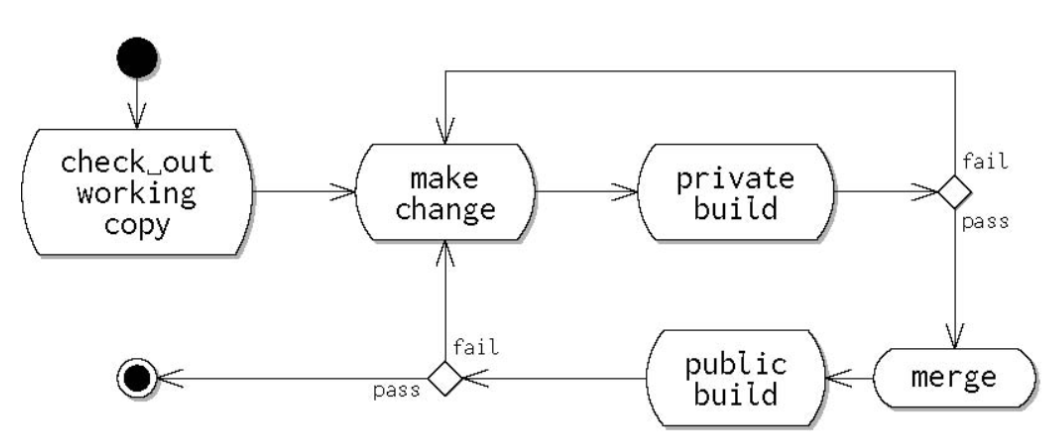
\includegraphics[scale=0.45]{src/9.3 preventing broken builds.PNG}
\end{figure}
\noindent The image illustrates the workflow of a build. 
\begin{itemize}
    \item First, a working copy is made of the latest version of the project source code, e.g. by cloning the repository and checking out the appropriate branch for the development effort. 
    \item Then, a change can be made to that code and a private build is performed on that change. That build should comprise of checks that would be applied to the production environment such as compiling the code, running tests and running any appropriate static analysis checks.
    \item If the build fails, then the developer should return to making changes and retesting the build using the build process. If the changes pass, the code should then be merged back into the master branch, where a public build is immediately performed.
    \item If the build passes, then all changes are finished and the process ends.
    \item If a broken build is detected at this stage, the development will need to review changes and immediately take the necessary steps to return the repository back to a functioning state.
\end{itemize}

Some development teams use feature branching and apply CI pipeline to each feature branch in code. This means that, in addition to the process described above, the development must take the additional step as shown below.
\begin{figure}[H]
    \centering
    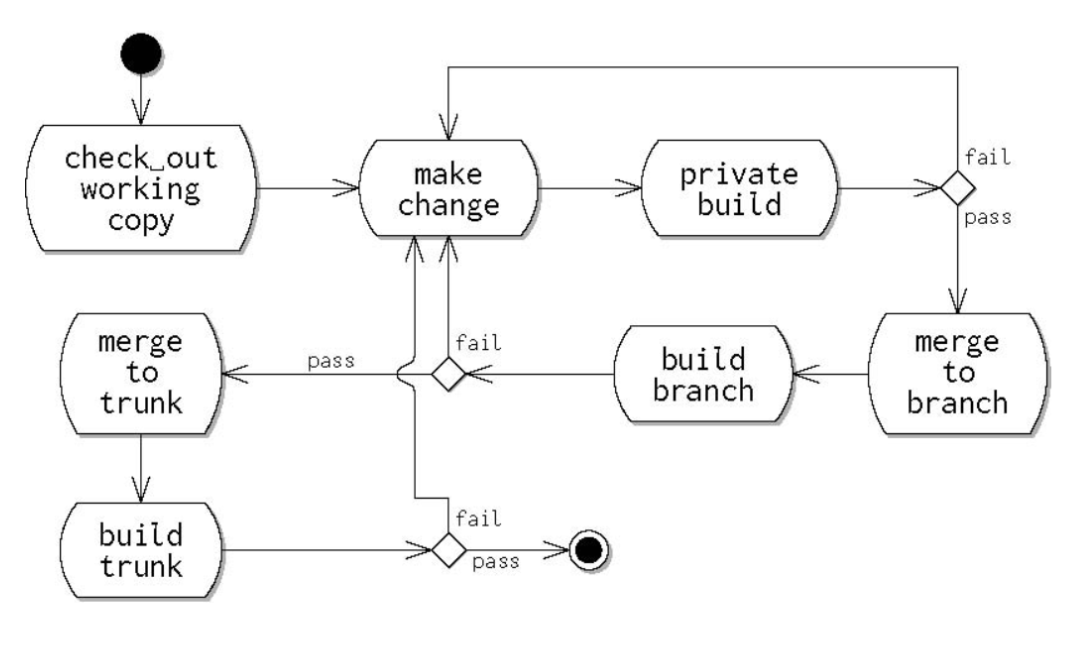
\includegraphics[scale=0.45]{src/9.4 preventing broken builds with branches.PNG}
\end{figure}

We first develop a feature in a branch. Next, we merge the latest changes from trunk into branch. We perform a successful build on the branch. Finally, we merge changes from the branch into trunk and perform successful build on trunk.

Although this approach can reduce the number of broken builds, it may also have the adverse effect of reducing the frequency of commits as well as making the size of a single commit larger. This is because the amount of effort required to integrate a new feature. This makes it less attractive to perform this task frequently.

\section{Staging Environments}
Changes to the software need to be checked before they are released to a wider userbase in order to gain assurance that any proposed change doesn't introduce any additional defect. 

A staging platform is an environment configured to replicate and simulate conditions a software it will be used in. It can be used to test software before it is released to the users. Staging platforms are configured with current hardware and software dependencies of the current baseline of the software.

Sometimes, it may be necessary to have more than one staging environment. The system may be compromised of several different distributed components, each of which are intended to be used on a different software platform. It is also possible for the same component to be executed on different platforms.

It is not always possible to build a staging environment that is an exact replica of production. This may be because:
\begin{itemize}
    \item the scale of the system in production is simply too large to replicate on too many computing nodes within a staging environment.
    \item the system may be used on too many different platforms or platform configurations to possible test all the different combinations.
    \item the system may have too many simultaneous users in order to be tested plausibly.
    \item there may be too many user types to be tested within the staging environment.
    \item there may only be one platform where the software is available and it is used for production.
    \item software dependencies, such as network end points and datasets cannot be accessed from outside the production.
\end{itemize}

\section{Continuous integration environment workflow}
\begin{figure}[H]
    \centering
    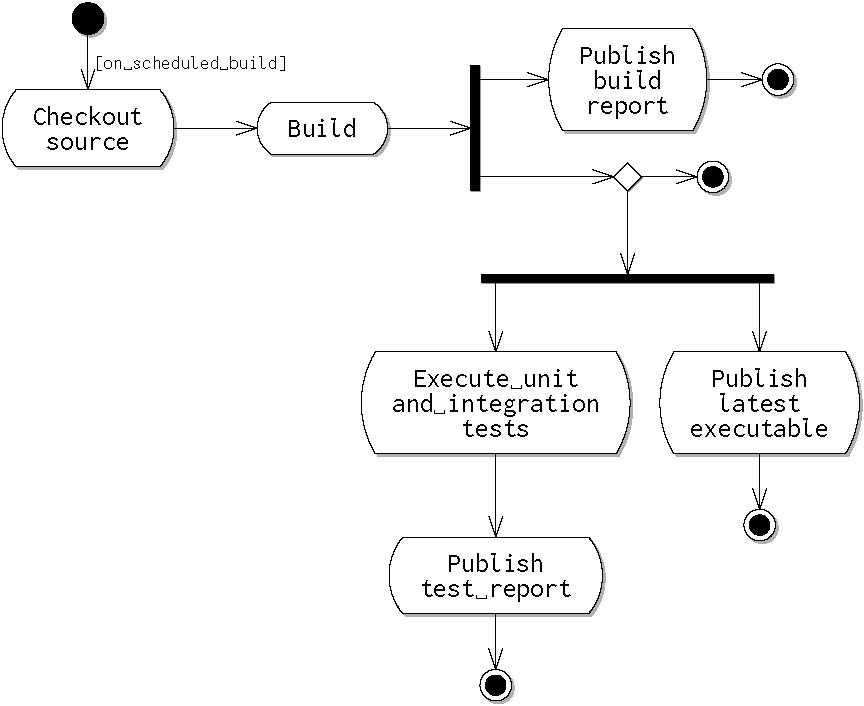
\includegraphics[scale=0.65]{src/9.5 continuous integration environment workflow.png}
\end{figure}
The diagram illustrates the workflow of a continuous integration environment for a typical job or pipeline. The code is checked out as a scheduled built on a new commit. The code is compiled and report published indicates whether the process was successful. If it is successful, unit and integration tests are applied to the compiled code and test report published. The latest executable will also be published.

In some cases, the pipeline may be configured to run the tests before the latest executable is published. This prevents executables that fail tests from being published.

\subsection{Maintaining Visibility}
As a project progresses, it is useful to find ways to disseminate information about the status of different associated processes. Common ways of disseminating information include push notifications and broadcast mechanisms, e.g. a status monitor. Useful metrics that may be sent are the following.
\begin{itemize}
    \item Statistical analysis of a number of unsuccessful builds over the previous period. It measures how frequently a project is broken due to integration values. 
    \item Also, average unsuccessful tests over a period can be measured. The build can be used to estimate the rate at which defects are being introduced into a project by the implementation of new features.
    \item Time to build can also be useful as a metric in order to measure and monitor how long a continuous integration process remains viable. The builds that take too long will deter software developers making frequently commits.
\end{itemize}

Fast builds are important for a successful continuous integration process. This is for 2 reasons:
\begin{itemize}
    \item Delays in completing a build will delay discovery of problems. So, A developer may continue working while a build is still in progress without realising that they have broken the current build.
    \item Developers may also be deterred from making frequent commits. They may not be able to make progress until they learn whether their previous commit has passed, and failed the build.
\end{itemize}

Advocates for continuous integration, as well as the extreme programming agile practice, recommend a maximum build time of 10 minutes. Unfortunately, as a project becomes larger, it may become more and more difficult to ensure that the build time remains acceptable.

This compromise can take several forms:
\begin{itemize}
    \item the team can look at re-configuring the build process to ensure that no unnecessary steps are being taken when a component is built. It may be that some optimisations are possible, which don't reduce the rigor of the quality checks performed.
    \item the team may also be able to configure several different types of builds that are performed for different parts of the project and causes of change. Changes that don't affect the published or public API of a class or a component may only need to trigger a build for a subsystem. Daily builds of the complete system can test the effects of all changes over a day.
    \item the team might also consider using strategies to prioritise test cases and partition them into different categories for different types of builds. The selection of an appropriate test cases for this regression test suite must compromise between efficiency. This completes the builds within 10 minutes and tests effectiveness in detecting the introducing of new defects. The selection of tests will need to be continually reviewed as new features are added, requiring more tests.
    \item the team partitions larger projects into smaller well-defined components that can be developed concurrently. Some components will then become dependencies of larger system. When a development change is made, only the components that are affected will need to be built and re-tested. Dependent components will not be affected until the change in dependency is reflected in a release. This is often good practice to ensure that a software project remains manageable.
\end{itemize}

\section{Advanced Topics}
\subsection{Continuous deployment}
A team that has completely automated the process of integrating the software project may also have the opportunity to extend the automation to delivery of software to users and customers. There are 2 main advantages to this.
\begin{itemize}
    \item It ensures the deployment process is regularly used. This means that the risk of deploying a new software release is lower. The process is automated, so it is better understood. Moreover, it will also probably encompass an automated process for rolling back a new deployment.
    \item Continuous deployment also creates the possibility of creating different feature variants to different subsets of users. This allows for techniques to be used, such as A/B testing.
\end{itemize}

\subsection{Chaos Engineering}
Rather than using quality assurance checks to prevent the introduction of defects, in chaos engineering, defects and failures are deliberately introduced into the production environment of the software system. This allows us to understand how the large scale software infrastructure copes with those failures and outages.

In summary, continuous integration practices minimise the disruption caused by rapid, concurrent changes to the software system. Software development projects routinely experience rapid concurrent change. This happens as many contributors fix defects and implement new features.

Integrating these changes at the end of the project iteration can be costly and difficult. Moreover, they can introduce unexpected delays to the project schedule. Continuous integration is a collection of practices that are designed to minimise this disruption to a project. In addition, continuous integration practices cover a mechanism for actively monitoring the quality of a software system as it evolves.

\end{document}